\chapter{Evaluation and Results} \label{chap:Evaluation and Results}

\section{Experiment Environment}

We evaluated our algorithm by building an adhoc cluster in AWS. We
have used Mesos as our resource manager for our cluster. Our compute
cluster has one mesos master node which is used
primarily to monitor slave nodes and do resource scheduling.
It also runs a spark history server. This node is not used for any computation.
We have ten slave nodes where all the computation happens. Each slave node has
8 vCPUs, 16 GB RAM and 80 GB Hard disk. The master node has 8 vCPUs,
16GB RAM and 80 GB Hard disk. Each vCPU is approximately 1/2 a
core. vCPU is unit used by AWS. All the nodes are running ubuntu as
base OS.

We performed experiments on two real datasets. We have run all our
experiments on both the datasets. We have found that the results are
consistent on both the datasets for all our experiments.

\begin{enumerate}
\item \textbf{Higgs Dataset:}
Higgs Dataset contains 28 features. These features are kinematic
properties measured by the particle detectors in the
accelerator. Classes are signal process which produces Higgs boson and
background process which does not. The dataset contains 11 Million
vectors with classes. The total size of the dataset file is 7.7 GB

\item \textbf{Forest Dataset:}
Forest Dataset is a real dataset which predicts the cover type of
forest from cartographic variables. It has 6 different classes. Each
vector has 54 attributes. Out of 54 only the first 10 are integer
attributes and rest are binary. we have used only first 10 attributes
in our tests. The dataset is relatively small and contains only 580K
vectors with classes. The total size of the datset file is 80 MB
\end{enumerate}

We will compare the results of our algorithm with brute force
algorithm. There are no known implementation available for spark and
there are no working implementation of any algorithm for any other
distributed framework. Due to this we study our algorithm performance
against bruteforce only.

\begin{minipage}{\linewidth}
In our experiments we have analysed the effect of the following variables on the
overall runtime, shuffle data and RAM utilization
\begin{enumerate}
\item Size of the dataset
\item Number of Neighbours (k)
\item Number of pivots
\item Number of compute Nodes
\item Number of dimensions
\end{enumerate}
\end{minipage}

\section{Effect of size of dataset}

In this section we will study the effect of size of the dataset on overall running
time and network bandwidth. We have compared the results against bruteforce algorithm.
We have used Higgs Dataset with 6 dimensions. In this experiment we
have utilized the entire ten node cluster for both bruteforce and our
algorithm.

\cref{fig_effect_of_dataset_size_1} shows how
the running time of the algorithm changes when the dataset increases.
Our proposed algorithm completed the 1 Million vector self join
in 2.2 minutes where as the brute force algorithm took about 3.9
hours. We are getting approximately 100 times faster even with the small
dataset.As the dataset size increases to 11 Million vectors, our
algorithm completed within 26 minutes.For brute force algorithm we can see that as the dataset doubles the running time
increases quadratically.  Due to this, we did not run the bruteforce
algorithm in such a large dataset as time taken will be too long. But
based on the quadratic increase we have seen as we double the data, our algorithm will be in comparison with
brute force about 800 to 1000 times faster for 11 Million x 11 Million.

\cref{fig_effect_of_dataset_size_2} shows the amount of data
shuffled between two nodes during the execution of the algorithm in
the cluster. The shuffle data includes both read and
write data. We can see that for our algorithm the shuffle bytes is
about 10 times lower than than the brute force. This shows our
algorithm is network bandwidth efficient.

We have used a total of 8.6 GB of RAM for storing all the datasets and
intermediate results while we ran the
algorithm. This is the total space used in all the slave nodes. It is
roughly equivalent to 900 MB of space usage per node. This is
equivalent to brute force algorithm.

\begin{figure*}[t!]
  \begin{subfigure}[t]{0.5\textwidth}
    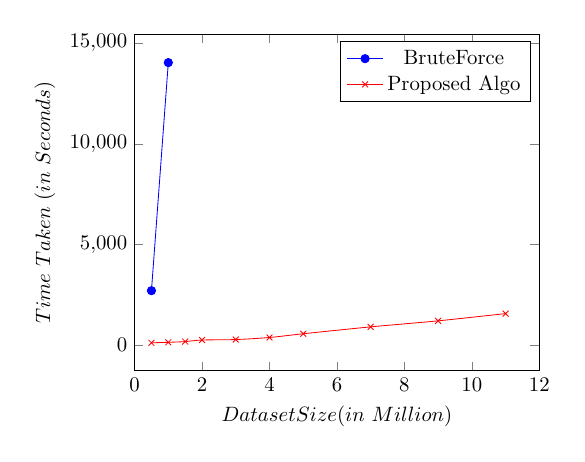
\begin{tikzpicture}[scale=0.75]
      \begin{axis}[
        xlabel=$Dataset Size(in\ Million)$,
        scaled x ticks = false,
        scaled y ticks = false,
        xmin=0, xmax=12,
        ylabel=$Time\ Taken\ (in\ Seconds)$]
        \addplot[smooth,mark=*,blue] plot coordinates {
          (0.5, 2700)
          (1, 14040)
        };
        \addlegendentry{BruteForce}

        \addplot[smooth,color=red,mark=x]
        plot coordinates {
          (0.5, 108)
          (1, 132)
          (1.500, 168)
          (2.000, 246)
          (3.000, 270)
          (4.000, 372)
          (5.000, 558)
          (7.000, 900)
          (9.000, 1200)
          (11.000, 1560)
        };
        \addlegendentry{Proposed Algo}
      \end{axis}
    \end{tikzpicture}
    \caption{on total runtime}
    \label{fig_effect_of_dataset_size_1}
  \end{subfigure}
  ~
  \begin{subfigure}[t]{0.5\textwidth}
  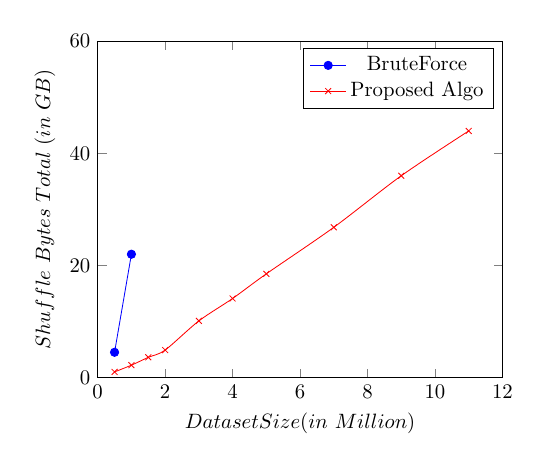
\begin{tikzpicture}[scale=0.75]
    \begin{axis}[
      xlabel=$Dataset Size(in\ Million)$,
      scaled x ticks = false,
      scaled y ticks = false,
      xmin=0, xmax=12,
      ymin=0, ymax=60,
      ylabel=$Shuffle\ Bytes\ Total\ (in\ GB)$]
      \addplot[smooth,mark=*,blue] plot coordinates {
        (0.5, 4.5)
        (1, 22)
      };
      \addlegendentry{BruteForce}

      \addplot[smooth,color=red,mark=x]
      plot coordinates {
        (0.5, 1)
        (1, 2.2)
        (1.500, 3.6)
        (2.000, 4.9)
        (3.000, 10.1)
        (4.000, 14.1)
        (5.000, 18.5)
        (7.000, 26.8)
        (9.000, 36.0)
        (11.000, 44.0)
      };
      \addlegendentry{Proposed Algo}
    \end{axis}
  \end{tikzpicture}
  \caption{on shuffle bytes}
  \label{fig_effect_of_dataset_size_2}
  \end{subfigure}
  \caption{Effect of dataset size}
  \label{fig_effect_of_dataset_size}
\end{figure*}

\section{Effect of k}

In this section we will study the effect of k on overall running
time and network bandwidth. We have compared the results against bruteforce algorithm.
We have used Higgs Dataset with 6 dimensions. In this experiment we
have utilized the entire ten node cluster for both bruteforce and our
algorithm. In order for us to compare against bruteforce algorithm we are using
500K vectors only.

\cref{fig_effect_of_k_1} shows how
the running time varies when the k increases. We see that for
bruteforce the running time remains constant. This is because the
number of computation per vector remains the same for brute force
algorithm. Hence finding any amount of k does not
cause any change in the total run time. Whereas we see that the
running time increases with increase in k for our algorithm. This is
because of two reasons
\begin{enumerate}
\item More comparison per vector
\item More data to be shuffled due to more neighbours per vector
\end{enumerate}

There is more comparison per vector as k increases, because the distance between a vector to
farthest neighbour increases with increase in k. As this distance increases, for more
points we need to look for neighbours across the partition. This
increases the average number of distance computation per vector. Hence
increasing the overall run time. Since we are checking neighbouring
partitions for more vectors, there is lot more data shuffling than
with lower number of neighbours. This as well increases the overall
running time. But Even with k = 15 we see that our
algorithm run faster than brute force.

\cref{fig_effect_of_k_2} shows the amount of data
shuffled between nodes during the runtime. This includes both read and
write data. For brute force algorithm has
linear increase in shuffle bytes when we increase k. This is expected
because as we increase k we need to find k nearest neighbour within
each partition. This k neighbours per vector has to be shuffled to every
other partition so that we can update the results. This causes
increase in amout of shuffled read and write bytes.

\begin{figure*}[t!]
  \begin{subfigure}[t]{0.5\textwidth}
    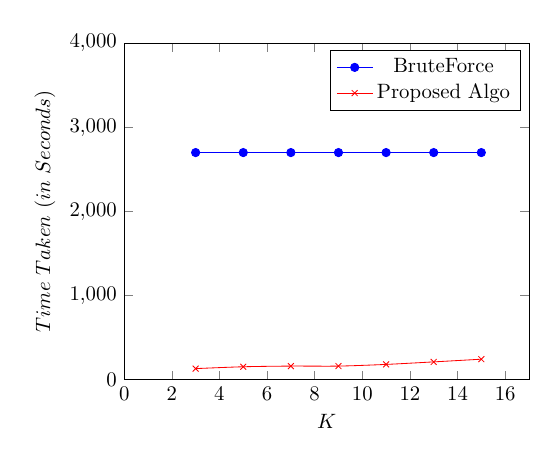
\begin{tikzpicture}[scale=0.75]
      \begin{axis}[
        xlabel=$ K $,
        scaled x ticks = false,
        scaled y ticks = false,
        xmin=0, xmax=17,
        ymin=0, ymax=4000,
        ylabel=$Time\ Taken\ (in\ Seconds)$]
        \addplot[smooth,mark=*,blue] plot coordinates {
          (3, 2700)
          (5, 2700)
          (7, 2700)
          (9, 2700)
          (11, 2700)
          (13, 2700)
          (15, 2700)
        };
        \addlegendentry{BruteForce}

        \addplot[smooth,color=red,mark=x]
        plot coordinates {
          (3, 130)
          (5, 152)
          (7, 160)
          (9, 160)
          (11, 180)
          (13, 210)
          (15, 242)
        };
        \addlegendentry{Proposed Algo}
      \end{axis}
    \end{tikzpicture}
    \caption{on total runtime}
    \label{fig_effect_of_k_1}
  \end{subfigure}
  ~
  \begin{subfigure}[t]{0.5\textwidth}
    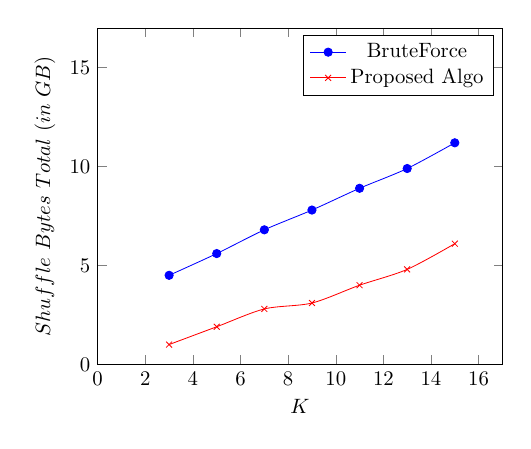
\begin{tikzpicture}[scale=0.75]
      \begin{axis}[
        xlabel=$ K $,
        scaled x ticks = false,
        scaled y ticks = false,
        xmin=0, xmax=17,
        ymin=0, ymax=17,
        ylabel=$Shuffle\ Bytes\ Total\ (in\ GB)$]
        \addplot[smooth,mark=*,blue] plot coordinates {
          (3, 4.5)
          (5, 5.6)
          (7, 6.8)
          (9, 7.8)
          (11, 8.9)
          (13, 9.9)
          (15, 11.2)
        };
        \addlegendentry{BruteForce}

        \addplot[smooth,color=red,mark=x]
        plot coordinates {
          (3, 1.0)
          (5, 1.9)
          (7, 2.8)
          (9, 3.1)
          (11, 4.0)
          (13, 4.8)
          (15, 6.1)
        };
        \addlegendentry{Proposed Algo}
      \end{axis}
    \end{tikzpicture}
    \caption{on shuffle bytes}
    \label{fig_effect_of_k_2}
  \end{subfigure}
  \caption{Effect of K}
  \label{fig_effect_of_k}
\end{figure*}

\section{Effect of number of pivots}

In this section we will study the effect of num pivots on overall running
time and network bandwidth.
We have used Higgs Dataset with 6 dimensions. In this experiment we
have utilized the entire ten node cluster for our
algorithm. To study the effect of pivots we are using dataset with 7
Million vectors. We are not comparing against bruteforce because this
is specific for our algorithm.

\cref{fig_effect_of_num_pivots_1} shows how
the running time varies when we change the number of pivots. Choosing
a right amount of pivot is important for our algorithm. Choosing a
value too high or too low results in longer running time of our
algorithm. This is clearly shown in the V shaped graph we got in our
tests. If the number of pivots is low, which means number elements per
partition is high. Since we are doing a join within a partition, this
will result in increase in number of distance computation per
vector. This inturn will result in increase in overall run time. If
the number of pivots is high, which means number of elements per
partition is low. This means more elements will not have neighbours
found within a single partition. This increases number of
shuffle. Moving data across partition has network overhead as well as
computation overhead. This causes increase in overall run time.
Empirically we have found that if the partition has elements between
1500 to 3000 then we have found right number of pivots. So for example
if we have a million elements then choosing 400 to 800 pivots gives
good results.

\cref{fig_effect_of_num_pivots_2} shows how the shuffle bytes
increases with increase in number of pivots.

\begin{figure*}[t!]
  \begin{subfigure}[t]{0.5\textwidth}
    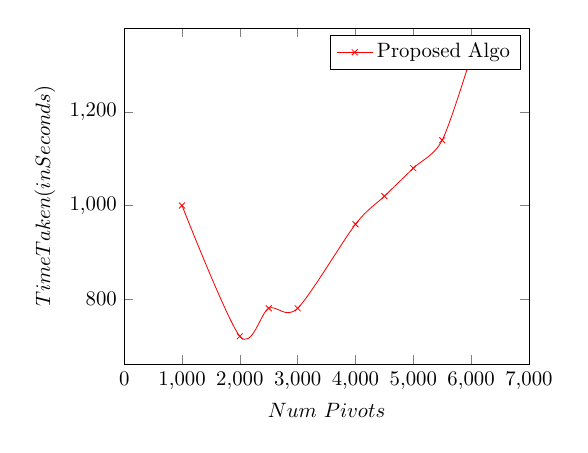
\begin{tikzpicture}[scale=0.75]
      \begin{axis}[
        xlabel=$Num\ Pivots$,
        scaled x ticks = false,
        scaled y ticks = false,
        xmin=0, xmax=7000,
        ylabel=$TimeTaken(inSeconds)$]

        \addplot[smooth,color=red,mark=x]
        plot coordinates {
          (1000, 1000)
          (2000, 720)
          (2500, 780)
          (3000, 780)
          (4000, 960)
          (4500, 1020)
          (5000, 1080)
          (5500, 1140)
          (6000, 1320)
        };
        \addlegendentry{Proposed Algo}
      \end{axis}
    \end{tikzpicture}
    \caption{on total runtime}
    \label{fig_effect_of_num_pivots_1}
  \end{subfigure}
  ~
  \begin{subfigure}[t]{0.5\textwidth}
  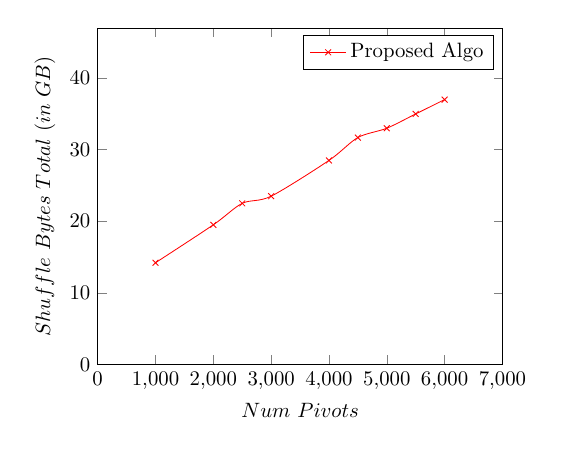
\begin{tikzpicture}[scale=0.75]
    \begin{axis}[
      xlabel=$ Num \ Pivots $,
      scaled x ticks = false,
      scaled y ticks = false,
      xmin=0, xmax=7000,
      ymin=0, ymax=47,
      ylabel=$Shuffle\ Bytes\ Total\ (in\ GB)$]
      \addplot[smooth,color=red,mark=x]
      plot coordinates {
          (1000, 14.2)
          (2000, 19.5)
          (2500, 22.5)
          (3000, 23.5)
          (4000, 28.5)
          (4500, 31.7)
          (5000, 33.0)
          (5500, 35.0)
          (6000, 37.0)
      };
      \addlegendentry{Proposed Algo}
    \end{axis}
  \end{tikzpicture}
  \caption{on shuffle bytes}
  \label{fig_effect_of_num_pivots_2}
  \end{subfigure}
  \caption{Effect of Number of Pivots}
  \label{fig_effect_of_num_pivots}
\end{figure*}


\section{Effect of dimensions}

In this section we will study the effect of number of dimension of a
vector on overall running time and network bandwidth.
We have used Higgs Dataset with 500k vectors. In this experiment we
have utilized the entire ten node cluster for our
algorithm. We have used small dataset so that we can compare with
brute force algorithm.

\cref{fig_effect_of_num_dim_1} shows how
the running time varies when we change the number of dimensions.
For brute force algorithm the
running time remains constant as number of computation almost remains the
same. For our algorithm, We see that as the number of pivots increases above 12 dimensions, the
overall running time increases steeply. This is solely due to curse of
dimensionality. As the dimensions increases, the points are equally
spread out in all dimensions \cite{beyer_when_1999}. This means for every vector we need more
partitions to be compared as most of the points lie on the edge of the
partition. This increases average number of computation per vector and
causes more shuffling of data. More shuffling is because vectors with
incomplete KNN needs to moved across multiple partitions to compute
the final KNN.

Even at 28 dimensions the
performance of our algorithm is much better than bruteforce. But if
the dimensions of the order 100, then it will be much better to use
bruteforce rather than our algorithm. Right now there is no algorithm
which can provide accurate KNN for higher dimension faster. There is a
potential scope for research work here.

\begin{figure*}[t!]
  \begin{subfigure}[t]{0.5\textwidth}
    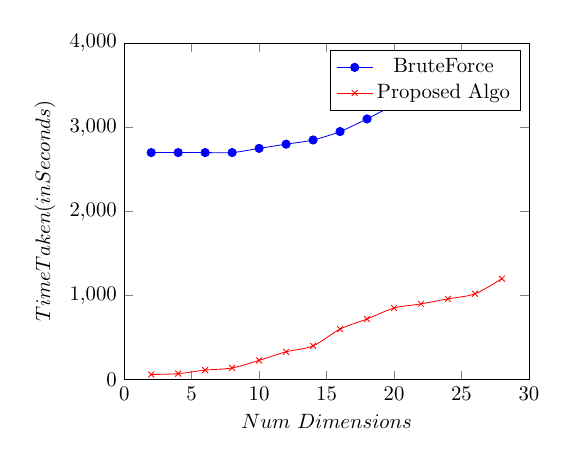
\begin{tikzpicture}[scale=0.75]
      \begin{axis}[
        xlabel=$Num\ Dimensions$,
        scaled x ticks = false,
        scaled y ticks = false,
        xmin=0, xmax=30,
        ymin=0, ymax=4000,
        ylabel=$TimeTaken(inSeconds)$]
        \addplot[smooth,mark=*,blue] plot coordinates {
          (2, 2700)
          (4, 2700)
          (6, 2700)
          (8, 2700)
          (10, 2750)
          (12, 2800)
          (14, 2850)
          (16, 2950)
          (18, 3100)
          (20, 3250)
          (24, 3400)
          (26, 3600)
          (28, 3700)
        };
        \addlegendentry{BruteForce}

        \addplot[smooth,color=red,mark=x]
        plot coordinates {
          (2, 60)
          (4, 70)
          (6, 112)
          (8, 138)
          (10, 228)
          (12, 330)
          (14, 400)
          (16, 600)
          (18, 720)
          (20, 850)
          (22, 900)
          (24, 960)
          (26, 1020)
          (28, 1200)
        };
        \addlegendentry{Proposed Algo}
      \end{axis}
    \end{tikzpicture}
    \caption{on total runtime}
    \label{fig_effect_of_num_dim_1}
  \end{subfigure}
  % ~
  % \begin{subfigure}[t]{0.5\textwidth}
  % \begin{tikzpicture}[scale=0.75]
  %   \begin{axis}[
  %     xlabel=$ K $,
  %     scaled x ticks = false,
  %     scaled y ticks = false,
  %     xmin=0, xmax=32,
  %     ymin=0, ymax=80,
  %     ylabel=$Shuffle\ Bytes\ Total\ (in\ GB)$]
  %     \addplot[smooth,mark=*,blue] plot coordinates {
  %       (2, 3.4)
  %       (4, 4.0)
  %       (6, 4.5)
  %       (8, 5.1)
  %       (10, 5.4)
  %       (12, 6.0)
  %       (14, 6.6)
  %       (16, 7.2)
  %       (18, 7.8)
  %       (20, 8.2)
  %       (22, 8.6)
  %       (24, 9.2)
  %       (26, 9.8)
  %       (28, 10.2)
  %     };
  %     \addlegendentry{BruteForce}

  %     \addplot[smooth,color=red,mark=x]
  %     plot coordinates {
  %       (2, 0.1)
  %       (4, 0.4)
  %       (6, 1.0)
  %       (8, 3.3)
  %       (10, 4.6)
  %       (12, 11.3)
  %       (14, 14.3)
  %       (16, 18.6)
  %       (18, 25.2)
  %       (20, 32.2)
  %       (22, 40.6)
  %       (24, 46.5)
  %       (26, 50.1)
  %       (28, 56.0)
  %     };
  %     \addlegendentry{Proposed Algo}
  %   \end{axis}
  % \end{tikzpicture}
  % \caption{on shuffle bytes}
  % \label{fig_effect_of_num_dim_2}
  % \end{subfigure}
  \caption{Effect of Number of Dimensions}
  \label{fig_effect_of_num_dim}
\end{figure*}

\section{Horizontal Scalability}
In this section we will study the scalability of our algorithm. We
will measure the running time and network bandwidth as we horizonally
scale.
We have used Higgs Dataset with 2M vectors with 6 dimensions. In this experiment we
have utilized the entire ten node cluster for our
algorithm.

\cref{fig_effect_of_num_nodes_1} shows how
the running time varies as we horizontally scale our cluster. Ideally,
Using distributed framework should help us achieve near linear
scalability. But once we reach a threshold the perfomance start to
remain constant because many nodes will not be used fully
utilized. This is observed in our results as well. In order to
optimize cost, one should rightly choose the number nodes so that we can have
faster results as well as low cost of running the cluster.

\cref{fig_effect_of_num_nodes_2} show that as we increase number of
nodes shuffle bytes increases. This is because for vectors whose
neighbours are in other partitions, vectors has to be shuffled to
right partition for computing the neighbours. As the number of nodes
increases data need to be shuffled to different nodes causing increase
in shuffle data.

\begin{figure*}[t!]
  \begin{subfigure}[t]{0.5\textwidth}
    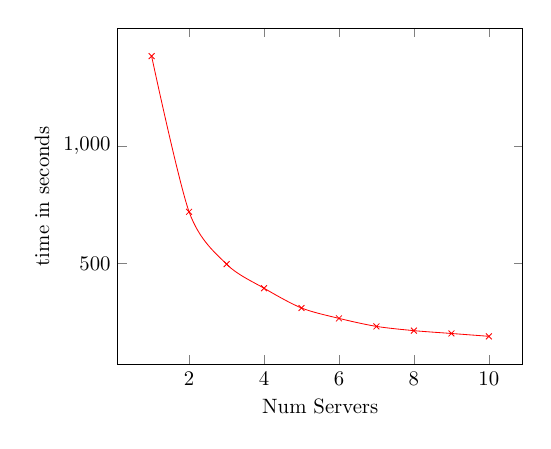
\begin{tikzpicture}[scale=0.75]
      \begin{axis}[
        % axis y line*=left,
        xlabel=Num Servers,
        ylabel=time in seconds,
        ]
        \addplot[smooth,color=red,mark=x]
        plot coordinates {
          (1, 1380)
          (2, 720)
          (3, 498)
          (4, 396)
          (5, 312)
          (6, 268)
          (7, 234)
          (8, 216)
          (9, 204)
          (10, 192)
        };
      \end{axis}
    \end{tikzpicture}
    \caption{on total runtime}
    \label{fig_effect_of_num_nodes_1}
  \end{subfigure}
  ~
  \begin{subfigure}[t]{0.5\textwidth}
  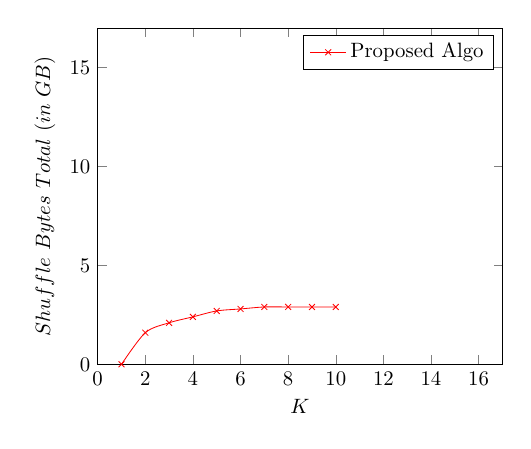
\begin{tikzpicture}[scale=0.75]
    \begin{axis}[
      xlabel=$ K $,
      scaled x ticks = false,
      scaled y ticks = false,
      xmin=0, xmax=17,
      ymin=0, ymax=17,
      ylabel=$Shuffle\ Bytes\ Total\ (in\ GB)$]

      \addplot[smooth,color=red,mark=x]
      plot coordinates {
        (1, 0)
        (2, 1.6)
        (3, 2.1)
        (4, 2.4)
        (5, 2.7)
        (6, 2.8)
        (7, 2.9)
        (8, 2.9)
        (9, 2.9)
        (10, 2.9)

      };
      \addlegendentry{Proposed Algo}
    \end{axis}
  \end{tikzpicture}
  \caption{on shuffle bytes}
  \label{fig_effect_of_num_nodes_2}
  \end{subfigure}
  \caption{Horizontal scalability}
  \label{fig_effect_of_num_nodes}
\end{figure*}

\bigskip
